\section{Architecture Frameworks}\label{sec:AAF}

%\subsection{Architecture Framework}\label{sec:archFram}

%\subsubsection{Overview}

An architecture framework is a
coordinated set of viewpoints, conventions, principles and practices
for architecture description within a specific domain of application
or community of stakeholders~\cite{42010}.  More specifically, it is determined by: (i) a set of architecture-related concerns,
(i) a set of stakeholders holding those concerns, (ii) a set of architecture viewpoints which frame (i.e.,
cover) those concerns, and (iv) a set of model correspondence rules to impose constraints between
types of models and then demonstrate that constraints
are satisfied by the architecture. 
%Then, an architecture framework establishes a common practice for creating, interpreting, analyzing and using architecture descriptions within a particular domain of application or stakeholder community, developing
%architecture modelling tools and architecting methods, and establishing processes to facilitate communication, commitments and interoperation across multiple projects and/or organizations~\cite{42010}.


%Uses of architecture frameworks include, but are not limited to~\cite{42010}: 
%
%\begin{itemize}
%\item creating architecture descriptions; 
%\item developing
%architecture modelling tools and architecting methods; 
%\item establishing processes to facilitate communication, commitments and interoperation across multiple projects and/or organizations.
%\end{itemize}

An architecture framework is a prefabricated knowledge structure, identified by {\em architecture viewpoints}, that
architects use to organize an architecture description into {\em architecture views}.  The terms architecture view and architecture viewpoint are central to the standard~\cite{42010}. 
%:
%``{\em A viewpoint is a way of looking at systems; a view is the result of applying a viewpoint to a particular
%system-of-interest}". 
An {\em architecture viewpoint} encapsulates notations, conventions, methods and techniques to
be used according to specific 
%model kinds framing particular
concerns and for a particular audience of system stakeholders. 
%The
%concerns determine what the model kinds must be able to express: e.g.,
%functionality, security, reliability, cost, deployment, etc.  %A model
%%kind determines the notations, conventions, methods and techniques to
%%be used. 
%%Viewpoints, defining the contents of each architecture view,
%%are built up from one or more model kinds and correspondence rules
%%linking them together to maintain consistency.
%%Viewpoints, like patterns and styles, are a form of reusable
%%architectural knowledge for solving certain kinds of architecture
%%description problems derived from best practices.  
%Viewpoints
%originated in the 1970s (in Ross' Structured Analysis) and refined in~\cite{Finkelstein+92}. Architecting methods often define one or
%more viewpoints, e.g.~\cite{4+1,RozWooBook,ClementsBachmannEtAl03, Eeles-Cripps:2010}.


Many existing practices express architectures through collections of
models, and models are further organized into cohesive groups, called {\em views}. A view can be defined as a ``{\em work product expressing the architecture of a system from the perspective of specific system concerns}"~\cite{42010}.
%As noted in the standard, the cohesion of a
%group of models is determined by specific concerns, which are addressed by that group of models. Viewpoints refer to the conventions
%for expressing an architecture with respect to a set of concerns.

For further discussion of the
content model and architecture frameworks mechanism,
see~\cite{Emery-Hilliard:2009}. 
%Recent
%frameworks include the ISO Reference Model for Open Distributed
%Processing, GERAM (Generalized Enterprise Reference Architecture
%and Methodology)~\cite{ISO15704}, DODAF (US Department of Defense Architecture
%Framework)~\cite{DODAF}, TOGAF~\cite{TOGAF}, and MODAF~\cite{MODAF}. 
For an extensive survey of
frameworks, see~\cite{AFS}. 
    


%\subsection{Automotive domain}\label{sec:automotiveAFs}

Architecture frameworks have not been standardized in the automotive domain and automotive industry. 
However, some attempts exist and different types of architecture viewpoints and views have been introduced recently as part
of automotive architecture frameworks.

%Automotive embedded systems are typically categorized into different domains, such as vehicle-centric functional domains
%(including powertrain control, chassis control, and active/passive safety systems) and
%passenger-centric functional domains (covering multimedia/telematics, body/comfort, and
%human machine interface (HMI))~\cite{Navet2008}. 
%Each functional domain needs to consider different stakeholders and
%system concerns~\cite{Yania}. %As an example, we can say that body domain supports the functioning of the airbag, wiper, and lighting
%%and other functions for the vehicle users, while the powertrain control enables the longitudinal propulsion
%%of the vehicle~\cite{Yania}). 
%However, at noted in~\cite{Yania} all the integrated functionalities must
%not jeopardize the key vehicle requirements of safety and efficiency.
%
%These considerations motivate the need of considering different viewpoints and views from the perspective of specific system concerns, which are relevant to one or more stakeholders. At the same time it is of key importance to identify and devise suitable connections among the various views and viewpoints.
%In other words, these considerations testify the need of an automotive architecture framework.

\patrizio{}

\section{State of the art in Automotive Architecture Frameworks}
A first attempt towards a standardized architectural foundation and automotive-specific
architecture framework is the Automotive
Architecture Framework (AAF) proposed in~\cite{Broy}. 
The purpose of AAF is to describe the entire vehicle system
across all functional and engineering domains and drive the thought process within the
automotive industry.
The AAF conforms to the ISO 42010 international standard~\cite{42010}, and therefore it is defined in terms of a set of viewpoints and views. 
%
%Figure~\ref{fig:aaf} shown the levels of architectures and architecture frameworks, spanning from the Meta Architecture Framework, which is the most generic layer that is fully independent of any type of system to develop, to the Product Architecture, which defines the architecture for a concrete product. 
%
  %
%\begin{figure}
%\begin{center}
%%  \vspace{-.3cm}
%  \includegraphics[width=.7\columnwidth]{figures/AAF.pdf}  
%  \caption{Automotive Architecture Framework (AAF) - Figure taken from~\cite{Broy}}
%%  \vspace{-.5cm}
%  \label{fig:aaf}
%    \end{center}
%\end{figure}
%
%Referring to~\cite{TUM-I0915}:
%
%The AAF is defined according to several levels; more details might be found at~\cite{TUM-I0915}. 
% of details as described below~\cite{TUM-I0915}:
%
%\begin{itemize}
%\item {\em Meta Architecture Framework} introduces terms like component, interface, view, viewpoint and concern. 
%\item {\em Common Architecture Framework} defines concepts, which are necessary for any kind of system. 
%%It is partitioned into three main parts, which are representing the total system at different layers of abstraction,
%%namely the Functional Architecture (functionality that the system offers
%% to its outside world - black-box and hardware agnostic), the Logical Architecture (decomposition of a system into a number of Logical Components - white-box and hardware agnostic) and the Technical Architecture (lower level of abstraction - runtime model, allocation, and hardware topology). 
%% % - see Figure~\ref{fig:abstractionDetails}.
%%\begin{itemize}
%%\item The Functional Architecture consists of a function hierarchy that contains the description of the functionality that the system offers
%% to its outside world. The description is black-box and is hardware agnostic. 
%%\item The Logical (Component) Architecture defines the decomposition of a system into a number of Logical Components, which interact
%%and cooperate to offer the functionality that is described in the Functional Architecture.
%%The description is then white-box, it can describe the functionality of a subsystem, and is hardware agnostic.
%%\item The Technical Architecture describes how the system that is specified by means of Logical Components can be integrated
%%into a given hardware platform. The system is presented from the  realization perspective. The technical architecture consists of three parts: The Runtime Model, the Allocation, and the Hardware Topology.
%%\end{itemize}
%\item {\em Domain-specific Architecture Framework for the Automotive Domain} defines the foundational framework providing a
%common denominator in terms of terminology, structure, methods, architecture models, guidance and rules. 
%%, ``{\em for
%%developing, representing, understanding, and comparing domain-specific product architectures across a
%%(virtual) development organization (i.e. Automotive value net)}"~\cite{TUM-I0915}.
%\item {\em Company X Architecture Framework} customizes the domain-specific Architecture
%Framework for a concrete company like Volvo cars, BMW or FIAT. We elaborate on the VCG architecture framework in Section~\ref{sec:VCGAF}.
%\item {\em Vehicle line architectures} defines the architecture for a specific product line.
%\item {\em Vehicle architectures} define the architecture for a specific product.
%\end{itemize}

 
%\begin{figure}
% \begin{center}
%%  \vspace{-.3cm}
%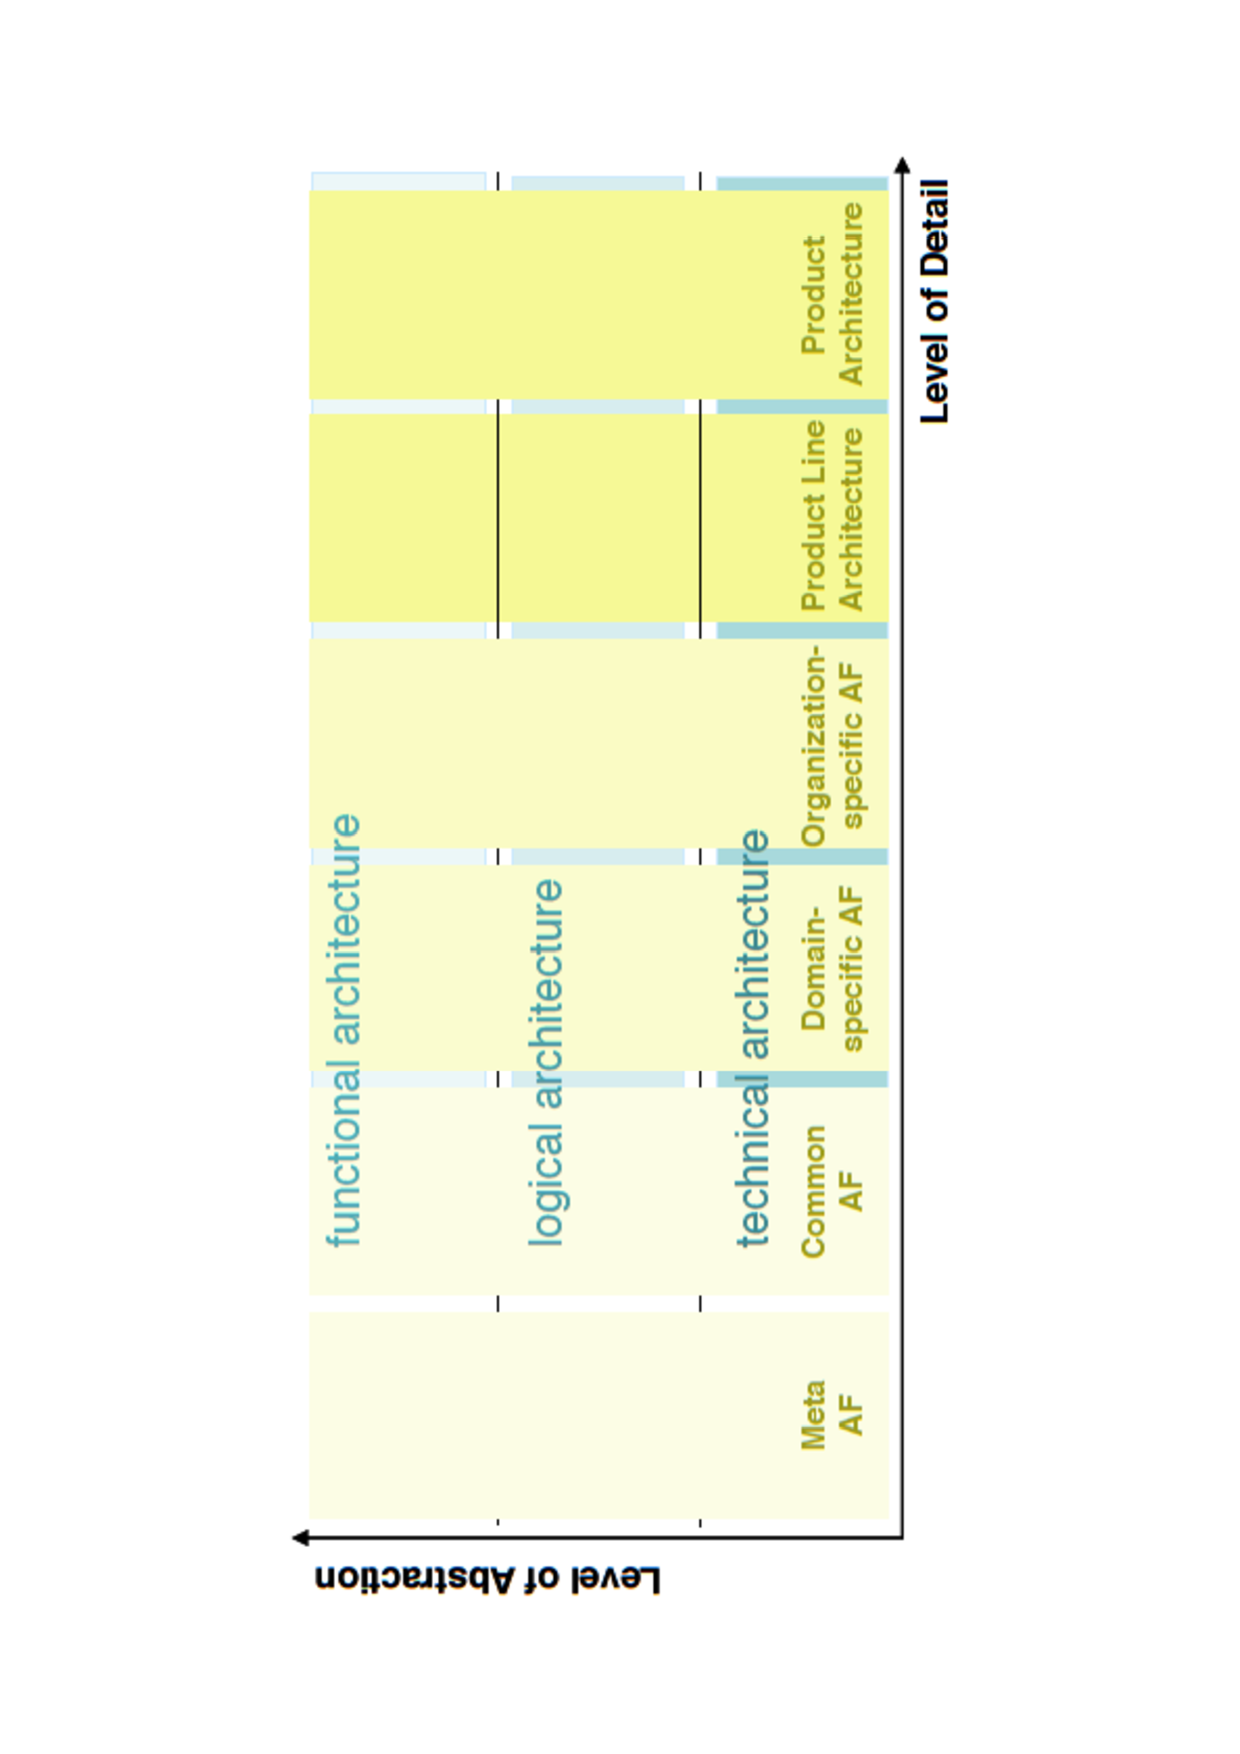
\includegraphics[width=6cm,angle=270]{figures/abstractionDetails.pdf}
%  \caption{Level of Abstraction and Level of Detail - Figure taken from~\cite{TUM-I0915}}
%%  \vspace{-.5cm}
%  \label{fig:abstractionDetails}
%      \end{center}
%\end{figure}


%Focusing on the Domain-specific Architecture Framework for the Automotive Domain, t
The AAF distinguishes between two sets of architecture viewpoints and views: (i) mandatory and general viewpoints and (ii) optional viewpoints. The following viewpoints are presented according to the viewpoint catalog in~\cite{Rozanski2005}.
The mandatory viewpoints and their respective views include: (i)
%
%\begin{itemize} 
%\item 
Functional viewpoint - functional decomposition, functional
architecture;
%\item 
(ii) Logical viewpoint - logical decomposition, logical architecture; this viewpoint is only mentioned in~\cite{Broy} but not detailed in~\cite{TUM-I0915};
%\item 
(iii) Technical viewpoint - physical decomposition, technical architecture;
%\item 
(iv) Information viewpoint - perspective of information or data objects used to
define and manage a vehicle;
%\item 
(v) Driver/vehicle operations viewpoint - vehicle environment;
%\item 
(vi) Value net viewpoint - OEM stakeholders and those of its suppliers and engineering partners. 
%\end{itemize}
The optional viewpoints suggested by the AAF are:
(i) Safety, (ii) Security, (iii) Quality and RAS - Reliability, Availability, Serviceability, (iv) Energy, possibly including performance, (v) Cost, (vi) NVH - noise, vibration, harshness, and (vii) Weight.

\subsection{Architectural Design Framework}

The Architectural Design Framework (ADF)~\cite{AFRenault} is developed by Renault %to support
%the construction of an architecture framework for the automotive industry. The ADF
and 
includes operational, functional, constructional, and requirements viewpoints. Although
the AAF and ADF are related they have some differences. 

\begin{itemize}
\item {\em Operational Viewpoint} - this is the more abstract viewpoint. %The actors, the system scope, the system environment and
%high-level interactions have to be identified; t
The system is observed from a black box and user perspective~\cite{AFRenault}.
\item {\em Functional  Viewpoint} - system functions %are obtained from 
identified in the views associated to the operational viewpoint %and by properly grouping or refining Activities (actions) and allocating them on 
are allocated to SysML Blocks. 
\item {\em Constructional Viewpoint} - this viewpoint %is more detailed and 
describes a further allocation (or grouping) of system functions into physical components.
\item {\em Requirements Viewpoint} - This viewpoint is orthogonal to other viewpoints. Each requirement view has a relationship with views of
other viewpoints. 
\end{itemize}

\subsection{Architecture Framework For Automotive Systems}
The Architecture Framework for Automotive Systems (AFAS) is proposed in~\cite{Yania} through an analysis of AAF, ADF and of Architecture Description Languages~\cite{ADL_Neno00,whatindustrywants} tailored to automotive domain, like EAST-ADL~\cite{EAST-ADL} %, TADL\footnote{TADL: Timing Augmented Description Language version
%2. \url{http://www.timmo-2-use.org/timmo/index.htm}.}, AADL~\cite{aadl}, 
and AML~\cite{AML}. 
It contains an elaboration and unification of the viewpoints proposed in AAF and ADF and then proposes additional viewpoints, e.g.:

\begin{itemize}
\item {\em Feature viewpoint} - to be used to support the product line engineering. %; it is inspired to~\cite{EAST-ADL}, the only automotive ADL supporting product lines in the architecture description.
\item {\em Implementation viewpoint} - 
it describes the software architecture of the Electrical/Electronic (E/E) system in the vehicle~\cite{EAST-ADL}. %, supported by the system architecture
%and software architecture of AUTOSAR. 
\end{itemize}


